\chapter{Fundamentação Teórica}\label{cap:fundamentacao_teorica}


As cadeiras de rodas motorizadas proporcionam conforto, segurança, rapidez e prevenção de lesões nos membros superiores devido ao uso repetitivo em cadeiras de rodas manuais. Porém, uma cadeira de rodas motorizada representa um alto custo: em uma análise do impacto orçamentário realizada pelo Departamento de Economia da Saúde, Investimento e Desenvolvimento- Ministério da Saúde-DESID/SE/MS, o preço sugerido para uma cadeira de rodas motorizada é de R\$ 4.999,00, além do custo de manutenção \cite{relatorio_sus}. Além disso, outro problema que as cadeiras de rodas motorizadas possuem é que em caso de necessidade, não podem ser usadas como cadeiras de rodas manuais, pois possuem rodas pequenas para aproveitar melhor a potência dos motores e sistema de transmissão. Outro detalhe importante é que cadeiras de rodas motorizadas são geralmente pesadas, e não possuem as facilidades de transportes das cadeiras manuais.


\section{Power Train}

\subsection{Motor}

	Motor é uma máquina que tem a capacidade de transformar energia elétrica em energia mecânica \cite{projeto_cadeira_rodas_inteligente}, existem dois tipos de motores, motor de corrente alternada (CA) e os de corrente contínua (CC).

	As cadeiras de rodas automáticas utilizam de baterias como fonte de alimentação para os motores, portanto se deve utilizar motores de corrente contínua. Este tipo de motor é muito utilizado em projetos que necessitam de velocidades variáveis, eles também apresentam uma região de torque e potência constante e são simples de realizar a aceleração e a desaceleração \cite{manual_bateria_unipower}.

	É necessário que as relações de velocidades entre os motores tenham um sistema de controle rígido de forma que o usuário consiga controlar a cadeira adequadamente. Os motores devem responder aos comandos sem que haja erros por uma questão de segurança. Uma metodologia para o dimensionamento de sistemas de tração para veículos elétricos é baseada na dinâmica veicular e considerando três condições de operação:

  \begin{itemize}
    \item Aceleração inicial
    \item Velocidade nominal
    \item Velocidade máxima
  \end{itemize}

	Um sistema que supre essas três condições funcionará adequadamente nos demais regimes de operação. Os parâmetros que definem essas restrições são:
  \begin{itemize}
    \item Velocidade nominal do veiculo
    \item Tempo especificado para o veiculo atingir a velocidade nominal
    \item Velocidade máxima
    \item Massa do veiculo
  \end{itemize}


	O objetivo é atender as restrições de projeto com o menor requerimento de potencia, ou seja, obter um perfil de torque-velocidade ótimo para o sistema de tração elétrica. Os motores de corrente continua utilizam das forças eletromagnéticas para transformar energia elétrica em mecânica, eles funcionam com uma fonte retificada, ou seja, que possuem polaridade fixa. Esse tipo de motor possui dois terminais, um positivo e outro negativo que de acordo com a polaridade e o sentido da corrente controlam a repulsão dos eletroímãs e consequentemente o sentido da rotação do motor.

	Uma das maiores vantagens dos motores de corrente continua é o controle da velocidade que é feito com o dreno de corrente para o motor. Porém são mais difíceis de serem construídos e mais propícios a problemas, gerando uma maior manutenção, além disso, são propícios a problemas com faíscas internas o que impede o seu uso em ambientes perigosos.


 \subsection{Bateria}
  Baterias são dispositivos que transformam energia química em elétrica e vice-versa. Por ser um processo reversível, as baterias podem ser carregadas e descarregadas várias vezes. Hoje no mercado existem vários tipos de baterias, com diferentes condições nominais.

  A bateria adequada ao projeto seria uma bateria de chumbo ácida, muito utilizada em veículos devido a seu fácil acesso e baixo custo. Atualmente ela já é utilizada em cadeiras de rodas elétricas. Este é o tipo menos eficiente de bateria, com a pior relação peso/energia, em compensação, é a tecnologia mais barata.

  Inventadas em 1859 pelo físico francês Gaston Planté, é muito utilizada hoje em dia em diferentes áreas, como automóveis, sistemas de fornecimento de energia elétrica ininterrupta (no-breaks) e cadeiras de rodas elétricas. Desprezando-se o problema do peso, é a bateria que mais se adéqua ao projeto

	Um grande problema foi solucionado na década de 70, onde pesquisadores conseguiram desenvolver uma bateria de chumbo-ácido livre de manutenção, podendo operar em qualquer posição. Nesta bateria, o invólucro foi selado e o eletrólito líquido foi transformado em separadores umedecidos.

	As baterias SLA (bateria selada chumbo-ácido), também conhecida como Gelcell, tem uma faixa típica de capacidade que vai de 0,2 Ah até 30 Ah. Esse tipo de bateria está livre do famoso efeito memória, e deixar a bateria em carga flutuante por um longo período não causa nenhum dano.

 	A bateria de chumbo-ácido tem a melhor retenção de carga entre todas as baterias recarregáveis. As baterias de SLA descarregam, em média, aproximadamente 40\% da sua energia armazenada em 1 ano, já uma de NiCd se auto descarrega na mesma quantidade em 3 meses.


  As baterias SLA devem sempre ser armazenadas carregadas. Deixar a bateria descarregada causa sulfação, uma condição que torna difícil, se não impossível, de se recarregar as baterias. A bateria SLA consegue fornecer entre 200 e 300 ciclos de carga/descarga.

    Vantagens:
    \begin{itemize}
      \item A mais barata em termos de custo por Watt horas;
      \item Segura e durável quando utilizada corretamente;
      \item Auto descarga está entre as mais baixas entre as baterias com sistema de recarga;
      \item Não exige muita manutenção e não tem o efeito memória.
    \end{itemize}

    Limitações:
    \begin{itemize}
      \item A bateria não pode ser armazenada em completa descarga, a tensão tem de estar acima de 2,10V;
      \item Densidade baixa da energia;
      \item Ciclo de carga/descarga limitado;
      \item O eletrólito e o conteúdo da carga podem causar danos ambientais;
      \item Imprópria para dispositivos de mão que exigem tamanho compacto.
    \end{itemize}

\subsubsection{Carregando Baterias}
  O tempo de carga de uma bateria de Chumbo-Ácido (selada) é de 12 a 16 horas. Com correntes de carga maiores, e métodos de carga multi-estágios, o tempo de carga pode ser reduzido para 10 horas ou menos. Durante a carga em corrente constante, a bateria carrega 70\% em aproximadamente 5 horas; os 30\% restantes são completados por uma lenta carga de pico. A corrente de pico dura outras 5 horas e é essencial para o bem estar da bateria.


\section{Controle}

Desde a primeira patente de cadeira de rodas elétrica em 1937 \cite{patent_cadeira_rodas_eletrica}, diversos modelos de cadeiras de rodas motorizadas foram desenvolvidos. As mais diversas interfaces humano-computador foram criadas de modo a facilitar a vida do cadeirante, desde cadeiras elétricas com um joystick simples à cadeiras inteligentes controladas por voz ou sem fio via celular, com monitoramento de velocidade, bateria e inclinação \cite{artigo_controle_cadeira_eletrica}. Foram pesquisas várias formas de controle de cadeiras de rodas que podem ser consultados na tabela \ref{tab:interfaces}.

\begin{table}[!htb]
\centering
\caption{Lista de dispositivos de controle de cadeiras de rodas elétricas.}
\begin{tabular}{|p{2cm}|p{3cm}|p{3cm}|p{4cm}|}
\hline
Interface & Comunicação & Monitoramento & Características \\ \hline
Joystick tradicional & Sem ou com fio, dependendo da aplicação. & Pouco, geralmente apenas o nível da bateria. & Contém mecanismo para encaixe na cadeira de rodas e ainda botões de emergência, os dados são enviados via bluetooth ou fio para o microcontrolador, onde é feito todo o processamento. \\ \hline
Joystick adaptado para o queixo & Com fio. & Nenhum. & Joystick fixo é adaptado para o controle com o queixo, utilizado por tetraplégicos. \\ \hline
Aplicativo em smartphone & Sem fio (VPN ou Bluetooth) & Total: nível da bateria, velocidade, inclinação e etc. & Um aplicativo de controle é instalado no celular, onde são mostradas as condições da cadeira e o usuário gera os comandos, todo o processamento é feito no microcontrolador, a aquisição e envio dos dados de monitoramento e as ações geradas pelo usuário. \\ \hline
Guidão e motor dianteiro & Mecânica. & Pouco ou nenhum. & Apenas para motores dianteiros. \\ \hline
\end{tabular}
\label{tab:interfaces}
\end{table}

\subsection{Dispositivos de controle}
Um mapeamento sobre uma maneira de implementação da cadeira de rodas automatizada pode ser observado na figura \ref{fig:diagrama_blocos}.

\begin{figure}[!htb]
\centering
  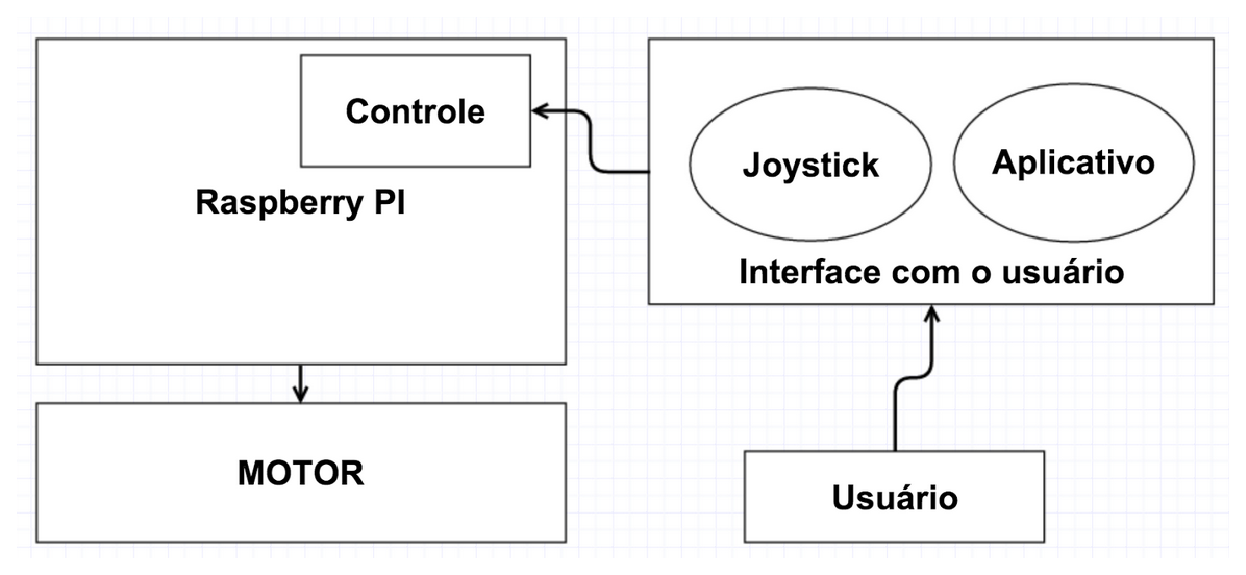
\includegraphics[keepaspectratio=true,scale=0.6]{figuras/controle/diagrama_blocos}
\caption{Desenho do diagrama de blocos de um sistema de controle simplificado para cadeiras de rodas automatizadas}
\label{fig:diagrama_blocos}
\end{figure}

Nesse esquemático pode ser observado que a interface com o usuário recebe uma entrada do usuário, utilizando-se um joystick ou aplicativo de celular. O sinal emitido por esta interface é então processado em um computador, a \textit{Raspeberry Pi} neste caso, que em seguida controla o movimento o motor.

\subsubsection{Joystick}
O joystick é um periférico de computador pessoal ou um dispositivo geral de controle que consiste em uma vara vertical na qual os pivôs se aproximam de uma extremidade e transmitem seu ângulo em duas ou três dimensões a um computador \cite{livro_creating_games}. O Joystick, muito utilizado em computadores e jogos eletrônicos provou sua utilidade em diversas áreas.

\subsubsection{Smartphones}
São dispositivos repletos de funções, tem uma grande portabilidade e sua facilidade de integração com outros sistemas é grande, dessa forma tornando-se uma possível solução para a interação do usuário com o sistema da cadeira de rodas.

\subsection{Tecnologias}

\subsubsection{Raspberry PI}

O Raspberry Pi é um computador do tamanho de um cartão de crédito que faz uso do sistema operacional Linux, foi desenvolvido para rodar aplicações de todos os tipos, internet, vídeo, dentre outras que geralmente rodam em um computador pessoal comum. Possui entradas USB que permitem a conexão de periféricos como mouse, teclado, câmeras e saídas para TVs como HDMI. Possui apenas memória volátil, sem disco rígido e roda o sistema operacional a partir de um cartão de memória \cite{rasp_foundation}.

O Raspberry Pi tem como principal componente um pequeno circuito integrado que reúne o processador com a arquitetura ARM, a GPU VideoCore IV e a memória RAM que é compativel com o sistema operacional GNU/Linux. As especificações gerais do modelo mais provável a ser utilizado no projeto, o \textit{Raspberry Pi Model B}, que pode ser visto na figura \ref{fig:rasp}, são:

\begin{itemize}
 \item Processador ARM 11 de 700 MHz;
 \item GPU VideoCore IV de 250 MHz;
 \item 256 MB total de RAM;
 \item Saída de vídeo HDMI e RCA;
 \item Saída de áudio P2;
 \item Interface de rede Ethernet;
 \item 2 portas USB;
 \item Conector Micro USB para alimentação (5 volts, 700mA).
\end{itemize}

\begin{figure}[!htb]
\centering
  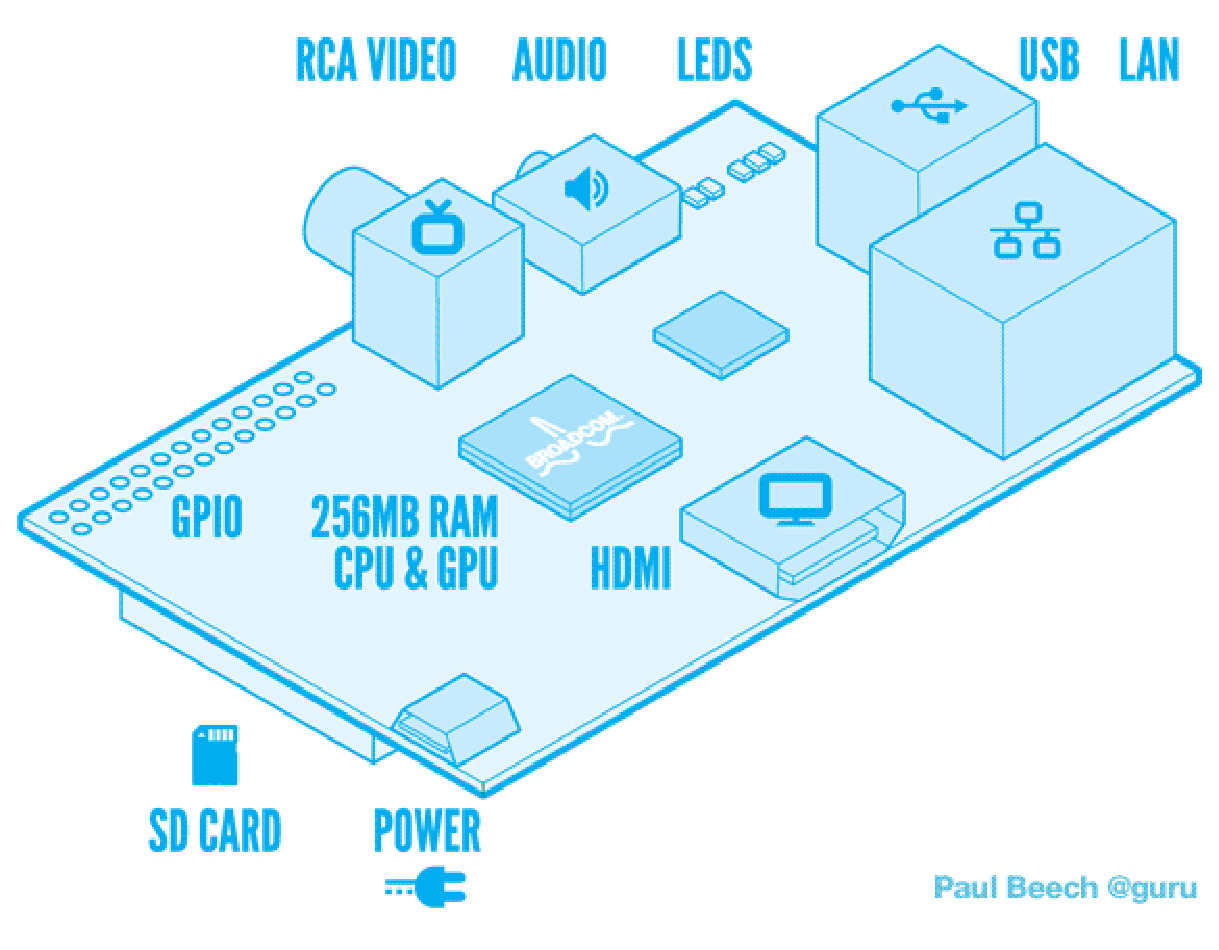
\includegraphics[keepaspectratio=true,scale=0.6]{figuras/controle/blueprint_rasp}
\caption{Esquemático componentes Raspeberry Pi}
\label{fig:rasp}
\end{figure}

\subsubsection{Python}

  Uma das linguagens a ser adotada será Python devido a facilidade de existir bibliotecas específicas que controlam o GPIO (General Purpose Input/Output) do Raspberry Pi.
  Essa linguagem é uma linguagem de programação de alto nivel, interpretada, orientada a objetos, de tipagem dinamica. Tem uma sintax consisa e clara, juntamente com uma biblioteca com recursos poderosos. Os módulos e frameworks ainda não foram decididos.

\subsubsection{Bluetooth}
  Bluetooth é um padrão de tecnologia de transmissão de dados sem fio para curtas distâncias, utilizando ondas de rádio UHF (de 2.4 à 2.485GHz \cite{bluetooth}). É utilizada pelos mais diversos dispositivos, como celulares, notebooks, desktops, sistemas embarcados, carros e etc, com esta tecnologia e possível conectar uma serie de dispositivos sem apresentar problemas de sincronização.

\subsection{Controle do motor}

  Geralmente motores precisam de corrente relativamente altas para controlar o seu funcionamento, assim é necessário que o sistema seja capaz de drenar corrente suficiente para os dispositivos. Considerando a característica dos motores de corrente continua, sua direção é controlada pelo sentido da corrente, pode-se construir um sistema para o controle do sentido de forma simples utilizando apenas chaves, transistores e o circuito de ponte H.
